\documentclass[10pt]{article}
\usepackage{kurzinfo}
\usepackage[table]{xcolor}
\usepackage{multirow}
\usepackage{longtable}
\usepackage{tabu}
\usepackage{ngerman}
\usepackage{lmodern}
\RequirePackage[ngerman=ngerman-x-latest]{hyphsubst}

\newcommand{\cmark}{\ding{51}}%
\newcommand{\xmark}{\ding{55}}%

\hyphenation{Haupt-bibliothek Informatik-zentrum Hörsaal-gebäude Seminar-gebäude}

\verantwortlich{M. Gehring} % HIER VISDP EINTRAGEN
\druck{AStA der RWTH}
\auflage{ca. 5000} %HIER APPROXIMIERTE AUFLAGE EINTRAGEN
\ausgabennummer{1} %% BITTE NACHSEHEN
\begin{document}
%<doppelseite>
%% DATUM KORRIGIEREN !!!%%%%

\newcommand{\mr}[2]{\multirow{-3}{*}{\parbox{#1}{\centering \hspace*{-.75ex} #2}}}

\begin{vorderseite}{Stand 05.02.2014}{Lernr\"aume} %erste Seite, Datum und Ueberschrift
\vspace{-1.5ex}
\begin{artikel}{\large Liebe Studis,}
\vspace{-2.0ex} {damit Ihr Euch w\"ahrend der vorlesungsfreien Zeit m\"oglichst in Ruhe auf eure Pr\"ufungen vorbereiten k\"onnt, haben wir in Zusammenarbeit mit der Zentralen Hochschulverwaltung eine Liste aller Lernr\"aume an der RWTH erstellt.Sollte es irgendwelche Probleme geben, so k\"onnt Ihr uns diese unter \email{lehre@asta.rwth-aachen.de} schildern und wir versuchen, sie schnellstm\"oglich zu beheben.\newline
\vspace{.2ex}\noindent
Wir w\"unschen Euch viel Erfolg bei den anstehenden Pr\"ufungen.\newline
\vspace{.2ex}\noindent
Euer AStA}
\end{artikel}
\vspace{-5ex}
{
\centering
\centering\setlength{\tabcolsep}{3pt}
\begin{longtabu} to 1.002\linewidth {|c|c|c|c|c|c|ccccc|X|}
\hline
\multirow{2}{*}{Gebäude} & \multirow{2}{*}{Adresse} & \multirow{2}{*}{Pl.} & \multirow{2}{*}{Raumbez.} & \multicolumn{2}{c|}{\multirow{2}{*}{Öffnungszeiten}} & \multicolumn{5}{c|}{\multirow{2}{*}{Ausstattung}} & \centering \multirow{2}{*}{\centering Bemerkungen}\\
&&&&\multicolumn{2}{c|}{~}&&&&&&\\\hline
\endfirsthead
\hline

\rg &&&& Mo - Fr & 09:00 - 22:00 &&&&&& \\
\rg &&&& Sa & geschlossen &&&&&& \\
\rg \mr{2.2cm}{SuperC} & \mr{2.5cm}{\href{http://maps.rwth-aachen.de/app/index.html?b=1040}{Templergraben 57}} & \mr{0.7cm}{268} & \mr{2.2cm}{Sparkassenforum} & So & geschlossen & \access & \wifi & \noethernet & \power & \nosilent & \\\hline

\rw &&&& Mo - Fr & 07:00 - 20:00 &&&&&& \\
\rw &&&& Sa & 07:00 - 20:00 &&&&&& \\
\rw \mr{2.2cm}{MOGAM} & \mr{2.5cm}{\href{http://maps.rwth-aachen.de/app/index.html?b=1060}{Kármánstr. 15a}} & \mr{0.7cm}{140} & \mr{2.2cm}{MOGAM} & So & 07:00 - 20:00 & \access & \wifi & \noethernet & \power & \nosilent & \mr{3.8cm}{\scriptsize \raggedright Raum 208 nicht barrierefrei}\\\hline

\rg &&&& Mo - Fr & 08:00 - 20:00 &&&&&& \\
\rg &&&& Sa & geschlossen &&&&&& \\
\rg \mr{2.2cm}{MOGAM} & \mr{2.5cm}{\href{http://maps.rwth-aachen.de/app/index.html?b=1060}{Kármánstr. 15a}} & \mr{0.7cm}{16} & \mr{2.2cm}{Korea-Treff} & So & geschlossen & \access & \wifi & \noethernet & \power & \nosilent & \mr{3.8cm}{\scriptsize \raggedright Betrieb durch Koreanische Studentenvereinigung (KSV)}\\\hline

\rw &&&& Mo - Fr & 07:00 - 20:30 &&&&&& \\
\rw &&&& Sa & geschlossen &&&&&& \\
\rw \mr{2.2cm}{Couven-Gymnasium} & \mr{2.5cm}{\href{http://maps.rwth-aachen.de/app/index.html?b=1070}{Kármánstr. 17~-~19}} & \mr{0.7cm}{24} & \mr{2.2cm}{Flur Anglistik} & So & geschlossen & \noaccess & \wifi & \noethernet & \nopower & \silent & \\\hline

\rg &&&& Mo - Fr & 08:00 - 22:00 &&&&&& \\
\rg &&&& Sa & geschlossen &&&&&& \\
\rg \mr{2.2cm}{HKW} & \mr{2.5cm}{\href{http://maps.rwth-aachen.de/app/index.html?b=1132}{Wüllnerstr. 1}} & \mr{0.7cm}{240} & \mr{2.2cm}{Foyer, HKW~3, HKW~4, HKW~5} & So & geschlossen & \access & \wifi & \noethernet & \power & \dash & \mr{3.8cm}{\scriptsize \raggedright Foyer, 5: Diskussionslernraum\newline 3, 4: Leiselernraum}\\\hline

\rw &&&& Mo - Fr & 08:00 - 24:00 &&&&&& \\
\rw &&&& Sa & 09:00 - 24:00 &&&&&& \\
\rw \mr{2.2cm}{Bibliothek 2} & \mr{2.5cm}{\href{http://maps.rwth-aachen.de/app/index.html?b=1160}{Templergraben 59}} & \mr{0.7cm}{160} & \mr{2.2cm}{BTH2} & So & 11:00 - 24:00 & \noaccess & \wifi & \ethernet & \power & \dash & \mr{3.8cm}{\scriptsize \raggedright 120 Pl. Leiselernraum\newline 40 Pl. Gruppenlernraum}\\\hline

\rg &&&& Mo - Fr & 08:00 - 24:00 &&&&&& \\
\rg &&&& Sa & 09:00 - 24:00 &&&&&& \\
\rg \mr{2.2cm}{Hauptbibliothek} & \mr{2.5cm}{\href{http://maps.rwth-aachen.de/app/index.html?b=1170}{Templergraben 61}} & \mr{0.7cm}{300} & \mr{2.2cm}{BTH} & So & 11:00 - 24:00 & \access & \wifi & \ethernet & \power & \silent & \mr{3.8cm}{\scriptsize \raggedright 3. OG laptopfrei}\\\hline

\rw &&&& Mo - Fr & 07:30 - 21:30 &&&&&& \\
\rw &&&& Sa & 09:00 - 14:00 &&&&&& \\
\rw \mr{2.2cm}{Audimax} & \mr{2.5cm}{\href{http://maps.rwth-aachen.de/app/index.html?b=1420}{Wüllnerstr. 9}} & \mr{0.7cm}{196} & \mr{2.2cm}{Flure, kleiner Lernraum} & So & geschlossen & \access & \wifi & \noethernet & \nopower & \nosilent & \mr{3.8cm}{\scriptsize \raggedright kleiner Lernraum: mit 230V-Anschluss}\\\hline

\rg &&&& Mo - Fr & 07:30 - 21:30 &&&&&& \\
\rg &&&& Sa & 09:00 - 21:00 &&&&&& \\
\rg \mr{2.2cm}{Audimax} & \mr{2.5cm}{\href{http://maps.rwth-aachen.de/app/index.html?b=1420}{Wüllnerstr. 9}} & \mr{0.7cm}{144} & \mr{2.2cm}{großer Lernraum} & So & geschlossen & \access & \wifi & \noethernet & \power & \nosilent & \\\hline

\rw &&&& Mo - Fr & 19:00 - 24:00 &&&&&& \\
\rw &&&& Sa & 08:00 - 24:00 &&&&&& \\
\rw \mr{2.2cm}{Semi90} & \mr{2.5cm}{\href{http://maps.rwth-aachen.de/app/index.html?b=1580}{Templergraben 90}} & \mr{0.7cm}{192} & \mr{2.2cm}{Semi90} & So & 08:00 - 24:00 & \access & \wifi & \ethernet & \power & \silent & \mr{3.8cm}{\scriptsize \raggedright in freien Zwischenzeiten auch als Lernraum nutzbar}\\\hline

\rg &&&& Mo - Fr & 09:00 - 19:00 &&&&&& \\
\rg &&&& Sa & geschlossen &&&&&& \\
\rg \mr{2.2cm}{Erweiterungsb. Architektur} & \mr{2.5cm}{\href{http://maps.rwth-aachen.de/app/index.html?b=1660}{Schinkelstr. 13}} & \mr{0.7cm}{196} & \mr{2.2cm}{Baumhaus} & So & geschlossen & \noaccess & \wifi & \noethernet & \power & \nosilent & \mr{3.8cm}{\scriptsize \raggedright Räume im EG barrierefrei}\\\hline

\rw &&&& Mo - Fr & 08:00 - 20:00 &&&&&& \\
\rw &&&& Sa & geschlossen &&&&&& \\
\rw \mr{2.2cm}{Seminargebäude} & \mr{2.5cm}{\href{http://maps.rwth-aachen.de/app/index.html?b=1810}{Wüllnerstr. 5b}} & \mr{0.7cm}{142} & \mr{2.2cm}{SG 202, SG 203, SG 413, SG 422} & So & geschlossen & \noaccess & \wifi & \noethernet & \nopower & \nosilent & \mr{3.8cm}{\scriptsize \raggedright nur eingeschränkte Barrierefreiheit; 202:~Leiselernraum}\\\hline

\rg &&&& Mo - Fr & 07:00 - 21:30 &&&&&& \\
\rg &&&& Sa & 07:00 - 14:00 &&&&&& \\
\rg \mr{2.2cm}{Kármán-Auditorium} & \mr{2.5cm}{\href{http://maps.rwth-aachen.de/app/index.html?b=1820}{Eilfschornsteinstr. 15}} & \mr{0.7cm}{84} & \mr{2.2cm}{Kármán-Foyer} & So & geschlossen & \access & \wifi & \noethernet & \power & \nosilent & \\\hline

\rw &&&& Mo - Fr & 07:00 - 21:30 &&&&&& \\
\rw &&&& Sa & 07:00 - 14:00 &&&&&& \\
\rw \mr{2.2cm}{Germanistisches Institut} & \mr{2.5cm}{\href{http://maps.rwth-aachen.de/app/index.html?b=1821}{Eilfschornsteinstr. 15}} & \mr{0.7cm}{72} & \mr{2.2cm}{Foyer, Verbindungsgang} & So & geschlossen & \access & \wifi & \noethernet & \power & \nosilent & \\\hline

\rg &&&& Mo - Fr & 08:30 - 17:30 &&&&&& \\
\rg &&&& Sa & geschlossen &&&&&& \\
\rg \mr{2.2cm}{Elektrische Nachrichtentechnik} & \mr{2.5cm}{\href{http://maps.rwth-aachen.de/app/index.html?b=2090}{Melatener~Str. 23~-~25}} & \mr{0.7cm}{47} & \mr{2.2cm}{IFHT} & So & geschlossen & \noaccess & \wifi & \noethernet & \nopower & \nosilent & \mr{3.8cm}{\scriptsize \raggedright Lernraum FB6: 10 PCs vorhanden}\\\hline

\rw &&&& Mo - Fr & 08:00 - 19:30 &&&&&& \\
\rw &&&& Sa & geschlossen &&&&&& \\
\rw \mr{2.2cm}{SB Bauingenieurwesen} & \mr{2.5cm}{\href{http://maps.rwth-aachen.de/app/index.html?b=2131}{Mies-v.d.Rohe-Str.~1}} & \mr{0.7cm}{16} & \mr{2.2cm}{Verbindung BauIng.} & So & geschlossen & \access & \wifi & \noethernet & \power & \silent & \\\hline

\rg &&&& Mo - Fr & 07:00 - 20:00 &&&&&& \\
\rg &&&& Sa & geschlossen &&&&&& \\
\rg \mr{2.2cm}{Hörsaalgebäude PPS} & \mr{2.5cm}{\href{http://maps.rwth-aachen.de/app/index.html?b=2315}{Prof.-Pirlet-Str.~12}} & \mr{0.7cm}{84} & \mr{2.2cm}{PPS Foyer} & So & geschlossen & \access & \wifi & \noethernet & \power & \nosilent & \\\hline

\rw &&&& Mo - Fr & 08:30 - 19:00 &&&&&& \\
\rw &&&& Sa & geschlossen &&&&&& \\
\rw \mr{2.2cm}{Informatikzentrum} & \mr{2.5cm}{\href{http://maps.rwth-aachen.de/app/index.html?b=2350}{Ahornstr.~55}} & \mr{0.7cm}{14} & \mr{2.2cm}{Hauptbau, 2022} & So & geschlossen & \access & \nowifi & \ethernet & \power & \silent & \\\hline

\end{longtabu}

}
\vspace{-6ex}
\end{vorderseite}


\begin{rueckseite}{Stand 05.02.2014}{Lernr\"aume} %Rueckseite, dass die immer so hei"st wie die Vorderseite, habe ich (noch) nicht hingekriegt.
\vspace{-3.5ex}
{
\centering
\centering\setlength{\tabcolsep}{3pt}
\begin{longtabu} to 1.000\linewidth {|c|c|c|c|c|c|ccccc|X|}
\hline
\multirow{2}{*}{Gebäude} & \multirow{2}{*}{Adresse} & \multirow{2}{*}{Pl.} & \multirow{2}{*}{Raumbez.} & \multicolumn{2}{c|}{\multirow{2}{*}{Öffnungszeiten}} & \multicolumn{5}{c|}{\multirow{2}{*}{Ausstattung}} & \centering \multirow{2}{*}{\centering Bemerkungen}\\
&&&&\multicolumn{2}{c|}{~}&&&&&&\\\hline
\endfirsthead
\hline

\rg &&&& Mo - Fr & 08:30 - 17:30 &&&&&& \\
\rg &&&& Sa & geschlossen &&&&&& \\
\rg \mr{2.2cm}{Informatikzentrum} & \mr{2.5cm}{\href{http://maps.rwth-aachen.de/app/index.html?b=2351}{Ahornstr.~55}} & \mr{0.7cm}{11} & \mr{2.2cm}{Foyer Schwimmbad} & So & geschlossen & \access & \nowifi & \noethernet & \nopower & \silent & \\\hline

\rw &&&& Mo - Fr & 08:30 - 17:30 &&&&&& \\
\rw &&&& Sa & geschlossen &&&&&& \\
\rw \mr{2.2cm}{Informatikzentrum} & \mr{2.5cm}{\href{http://maps.rwth-aachen.de/app/index.html?b=2352}{Ahornstr.~55}} & \mr{0.7cm}{44} & \mr{2.2cm}{Foyer Informatik} & So & geschlossen & \access & \wifi & \ethernet & \power & \silent & \mr{3.8cm}{\scriptsize \raggedright 24h-Zugang mittels Schlüssel gegen Kaution}\\\hline

\rg &&&& Mo - Fr & 08:30 - 17:30 &&&&&& \\
\rg &&&& Sa & geschlossen &&&&&& \\
\rg \mr{2.2cm}{Informatikzentrum} & \mr{2.5cm}{\href{http://maps.rwth-aachen.de/app/index.html?b=2353}{Ahornstr.~55}} & \mr{0.7cm}{48} & \mr{2.2cm}{Erweiterungsbau} & So & geschlossen & \access & \nowifi & \noethernet & \nopower & \silent & \\\hline

\rw &&&& Mo - Fr & 08:30 - 19:30 &&&&&& \\
\rw &&&& Sa & geschlossen &&&&&& \\
\rw \mr{2.2cm}{Informatikzentrum} & \mr{2.5cm}{\href{http://maps.rwth-aachen.de/app/index.html?b=2353}{Ahornstr.~55}} & \mr{0.7cm}{155} & \mr{2.2cm}{Bibliotheken} & So & geschlossen & \access & \wifi & \ethernet & \power & \silent & \mr{3.8cm}{\scriptsize \raggedright KiWi 4002 kleinkindergerecht}\\\hline

\rg &&&& Mo - Fr & 08:00 - 19:00 &&&&&& \\
\rg &&&& Sa & geschlossen &&&&&& \\
\rg \mr{2.2cm}{Informatikzentrum} & \mr{2.5cm}{\href{http://maps.rwth-aachen.de/app/index.html?b=2356}{Ahornstr.~55}} & \mr{0.7cm}{72} & \mr{2.2cm}{5054, 5055} & So & geschlossen & \access & \wifi & \noethernet & \power & \nosilent & \\\hline

\rw &&&& Mo - Fr & 08:00 - 17:30 &&&&&& \\
\rw &&&& Sa & geschlossen &&&&&& \\
\rw \mr{2.2cm}{Informatikzentrum} & \mr{2.5cm}{\href{http://maps.rwth-aachen.de/app/index.html?b=2356}{Ahornstr.~55}} & \mr{0.7cm}{72} & \mr{2.2cm}{Foyer, Garderobe} & So & geschlossen & \access & \wifi & \noethernet & \power & \silent & \\\hline

\rg &&&& Mo - Fr & 08:00 - 17:30 &&&&&& \\
\rg &&&& Sa & geschlossen &&&&&& \\
\rg \mr{2.2cm}{Büropark Aachen} & \mr{2.5cm}{\href{http://maps.rwth-aachen.de/app/index.html?b=3011}{Kackertstr.~7}} & \mr{0.7cm}{24} & \mr{2.2cm}{B~040, B~060, B~061} & So & geschlossen & \access & \wifi & \noethernet & \power & \silent & \\\hline

\rw &&&& Mo - Fr & 08:00 - 17:30 &&&&&& \\
\rw &&&& Sa & geschlossen &&&&&& \\
\rw \mr{2.2cm}{Aixtron A} & \mr{2.5cm}{\href{http://maps.rwth-aachen.de/app/index.html?b=3020}{Kackertstr.~15}} & \mr{0.7cm}{44} & \mr{2.2cm}{Se 3} & So & geschlossen & \access & \wifi & \noethernet & \power & \silent & \\\hline

\rg &&&& Mo - Fr & s. Aushang &&&&&& \\
\rg &&&& Sa & geschlossen &&&&&& \\
\rg \mr{2.2cm}{Rochusstraße} & \mr{2.5cm}{\href{http://maps.rwth-aachen.de/app/index.html?b=3990}{Rochusstr. 2~-~14}} & \mr{0.7cm}{134} & \mr{2.2cm}{Rochusstraße} & So & geschlossen & \noaccess & \wifi & \noethernet & \nopower & \nosilent & \mr{3.8cm}{\scriptsize \raggedright EG barrierefrei, RS~106:~Leiselernraum}\\\hline

\rw &&&& Mo - Fr & 08:30 - 17:30 &&&&&& \\
\rw &&&& Sa & geschlossen &&&&&& \\
\rw \mr{2.2cm}{Walter-Schottky-Haus} & \mr{2.5cm}{\href{http://maps.rwth-aachen.de/app/index.html?b=4243}{Sommerfeldstr. 24}} & \mr{0.7cm}{24} & \mr{2.2cm}{24 C 105} & So & geschlossen & \noaccess & \wifi & \noethernet & \power & \silent & \mr{3.8cm}{\scriptsize \raggedright eingeschränkt barrierefrei\newline wenn verschlossen: Fr. Jenkes öffnet}\\\hline

\rg &&&& Mo - Fr & 09:00 - 16:30 &&&&&& \\
\rg &&&& Sa & geschlossen &&&&&& \\
\rg \mr{2.2cm}{Sammelbau Physik} & \mr{2.5cm}{\href{http://maps.rwth-aachen.de/app/index.html?b=4281}{Sommerfeldstr. 16}} & \mr{0.7cm}{10} & \mr{2.2cm}{III. Physikalisches Institut} & So & geschlossen & \access & \nowifi & \ethernet & \nopower & \silent & \mr{3.8cm}{\scriptsize \raggedright 10 PCs vorhanden}\\\hline

\rw &&&& Mo - Fr & 07:00 - 19:00 &&&&&& \\
\rw &&&& Sa & geschlossen &&&&&& \\
\rw \mr{2.2cm}{Sammelbau Biologie} & \mr{2.5cm}{\href{http://maps.rwth-aachen.de/app/index.html?b=5421}{Worringer Weg~1}} & \mr{0.7cm}{12} & \mr{2.2cm}{Foyer SB Bio} & So & geschlossen & \access & \wifi & \noethernet & \power & \silent & \mr{3.8cm}{\scriptsize \raggedright 8 PCs vorhanden}\\\hline

\rg &&&& Mo - Fr & 07:00 - 19:00 &&&&&& \\
\rg &&&& Sa & geschlossen &&&&&& \\
\rg \mr{2.2cm}{Theaterplatz} & \mr{2.5cm}{\href{http://maps.rwth-aachen.de/app/index.html?b=6070}{Theaterplatz~14}} & \mr{0.7cm}{8} & \mr{2.2cm}{Flure} & So & geschlossen & \access & \nowifi & \noethernet & \nopower & \nosilent & \\\hline

\end{longtabu}

}
\vspace{2ex}
\zweispalten{.57\linewidth}%Breite der linken Spalte, der Kontaktblock sitzt im Stylefile\ldots
{
%\vspace{-8ex}
\fcolorbox{black}{light}{\parbox{\linewidth}{\textbf{Hinweise und Haftungsausschluss}%Beispielbox

{
\scriptsize 

\vspace{0.80ex}

Die angegebenen Öffnungszeiten sind mit der Hochschulverwaltung abgesprochen. Sollte es hier Probleme geben, wendet Euch bitte an \email{lehre@asta.rwth-aachen.de}.

\vspace{1.50ex}

Falls sich Fehler in die Liste eingeschlichen haben oder Informationen falsch sind, gebt uns bitte auch Bescheid.

\vspace{1.50ex}

Verbindliche Auskünfte erteilen die jeweils zuständigen Stellen. AStA und Redaktion haften nicht für die Inhalte dieses Informationsblattes.

}}}
}
{
\fcolorbox{black}{light}{\parbox{1.00\linewidth}{\textbf{Legende}%Beispielbox

\vspace{1.50ex}

\scriptsize\begin{tabu}{c|lc|l}

\includegraphics[height=1.5ex]{access}~   & barrierefrei        & 
\includegraphics[height=1.5ex]{noaccess}~   & nicht barrierefrei\\

\includegraphics[height=1.5ex]{wifi}~     & eduroam-Zugang      & 
\includegraphics[height=1.5ex]{nowifi}~     & kein eduroam-Zugang\\

\includegraphics[height=1.5ex]{ethernet}~ & Ethernet-Anschluss  & 
\includegraphics[height=1.5ex]{noethernet}~ & kein Ethernet-Anschluss\\

\includegraphics[height=1.5ex]{power}~    & 230V-Anschluss       & 
\includegraphics[height=1.5ex]{nopower}~    & kein 230V-Anschluss\\

\includegraphics[height=1.5ex]{silent}~   & Leiselernraum       & 
\includegraphics[height=1.5ex]{nosilent}~   & Diskussionslernraum
\end{tabu}

\vspace{1.50ex}
Piktogramme von The Noun Project}

}
}
\vspace{2ex}
\vfill\noindent
\fcolorbox{black}{light}{
\begin{minipage}[b]{0.993\linewidth}
\parbox{\linewidth}{
\parbox[t]{.25\linewidth}{
\scriptsize
\textbf{\footnotesize Kontakt zum AStA:}\\
Allgemeiner Studierendenausschuss \\
der RWTH Aachen\\
Peterstr. 44-46, 52062 Aachen\\
Tel.: 0241 / 80 - 93792 \\
Fax.: 0241 / 80 - 92394 \\
\url{http://www.asta.rwth-aachen.de/}\\
\email{asta@asta.rwth-aachen.de} \\
%\vspace*{7ex}
%\setlength\fboxsep{0pt}
%\setlength\fboxrule{0.5pt}
%\fbox{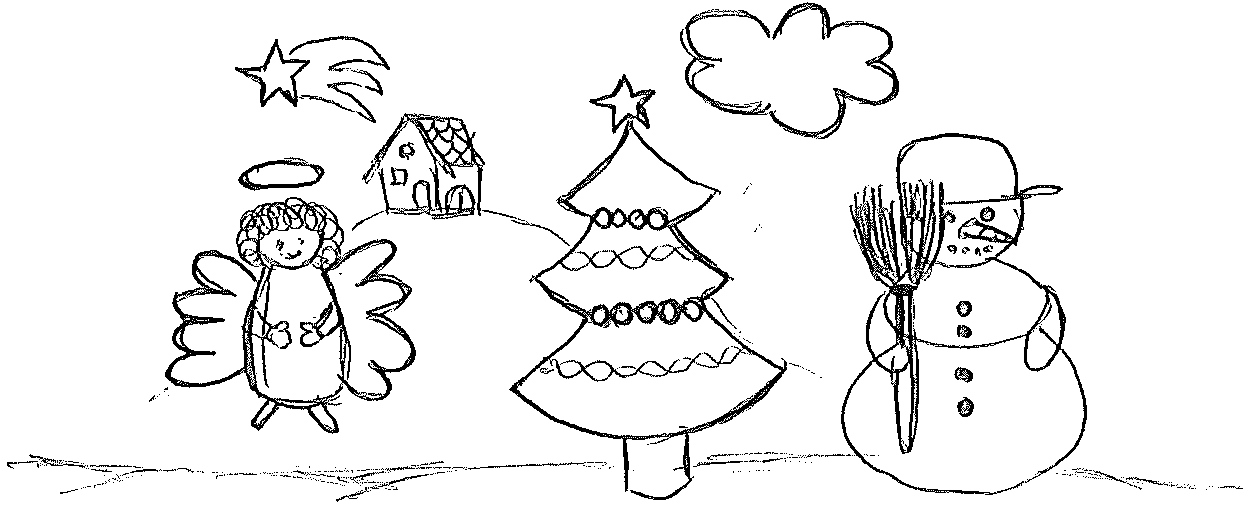
\includegraphics[scale=0.25]{/opt/share/90sek/Logos/Schneebild}} \\
%\vspace*{-11ex}
\\
\scriptsize
\textbf{\footnotesize \"Offnungszeiten:}\\
Mo. -- Fr. \hfill{} 10\Uhr{} -- 14\Uhr{} Uhr\hspace*{1ex}\\
\vspace*{0.2ex}

\textbf{\footnotesize AStA Sitzungen:}\\
\scriptsize Mo. 14\Uhr{} Uhr (nat\"urlich \"offentlich!)\\
}
\parbox[t]{.10\linewidth}{}
\parbox[t]{.28\linewidth}{

\textbf{\footnotesize Service-Zeiten:}\\
\scriptsize
Beglaubigung:           \hfill{} Mo. -- Fr. 10\Uhr{} -- 14\Uhr{} Uhr\hspace*{1ex}\\
ISIC:                   \hfill{} Mo. -- Fr. 10\Uhr{} -- 14\Uhr{} Uhr\hspace*{1ex}\\
AStA-Kultur:            \hfill{} nach Vereinbarung{}    \hspace*{1ex}\\
% \vspace*{0.2ex}
\\
\textbf{\footnotesize Rechtsberatung:}\\
Allgemein: \hfill{} nach Vereinbarung \\
Prüfungsrecht: \hfill{} nach Vereinbarung\\
Mietrecht: \hfill{} nach Vereinbarung\\
Ausländerrecht: \hfill{} nach Vereinbarung\\
\\
{\it Die Termine zur Rechtsberatung werden nur nach vorheriger Terminabsprache im AStA vergeben. \\(nicht telefonisch)}
}
\parbox[t]{.10\linewidth}{}
\parbox[t]{.45\linewidth}{

\raggedright{\textbf{\footnotesize Beratungszeiten:}}\\
\scriptsize
Wohnen:                         \hfill{}Mo., Mi., Do., Fr. 10\Uhr{} -- 14\Uhr{} Uhr                     \hspace*{1ex}\\

BAföG:                        \hfill{}Di., Mi, Do, Fr. 10\Uhr{} -- 14\Uhr{} Uhr             \hspace*{1ex}\\

Studienfinanzierung, Jobben:           \hfill{}Mi. \& Fr. 10\Uhr{} -- 14\Uhr{} Uhr             \hspace*{1ex}\\

Studieren mit Kind / Pflege:            \hfill{}Mo. 12\Uhr{} -- 14\Uhr{} Uhr                    \hspace*{1ex}\\
                                \hfill{}Do. 10\Uhr{} -- 14\Uhr{} Uhr                    \hspace*{1ex}\\

Sozialdarlehen und Beihilfen:   \hfill{}Mo. \& Mi. 10\Uhr{} -- 14\Uhr{} Uhr             \hspace*{1ex}\\
                                \hfill und nach Vereinbarung                            \hspace*{1ex}\\

Behinderung / chr. Krankheit:   \hfill{}Mo. 10\Uhr{} -- 12\Uhr{} Uhr                    \hspace*{1ex}\\
                                \hfill{}Di. 10\Uhr{} -- 14\Uhr{} Uhr                    \hspace*{1ex}\\
                                \hfill{}Do. 12\Uhr{} -- 14\Uhr{} Uhr                    \hspace*{1ex}\\
                                \hfill{}Fr. 10\Uhr{} -- 14\Uhr{} Uhr                    \hspace*{1ex}\\

Gleichstellung:                \hfill{}Mo. \& Fr. 10\Uhr{} -- 14\Uhr{} Uhr               \hspace*{1ex}\\

AV-Beratung (Humboldt-Haus): \hfill{}Mo. -- Mi., Fr. 10\Uhr{} -- 12\Uhr{} Uhr                  \hspace*{1ex}\\
\vspace*{-1.7ex}

}
}
%% Dies ist die letzte kleine schwarze Box auf der zweiten Seite. Wird in den jeweiligen Style-files eingebunden.
\vspace*{-1ex}

\rule{\linewidth}{.5pt}
\vspace*{-3.5ex}

\textbf{\scriptsize Impressum:}
{\footnotesize AStA der RWTH Aachen, Peterstr. 44-46, 52062 Aachen; ViSdP:  \visdp{}; \email{lehre@asta.rwth-aachen.de}; Auflage: 
\auflagenhoehe \hspace*{1ex}Stk. \hspace*{\fill}}
\end{minipage}
}

\vspace{-5ex}

%\begin{artikel}{Linkliste/Weitere Informationen}
\parbox{.1\linewidth}{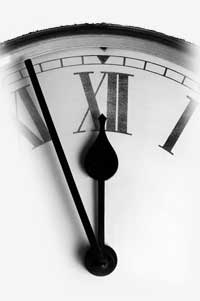
\includegraphics[width=\linewidth]{bilder/uhr}}
\parbox{.9\linewidth}{
\begin{aufzaehlung}
\item \url{www.asta.rwth-aachen.de} -- Webseiten des AStA mit aktuellen Infos und Sprechzeiten der BAf"oG-Beratung
\item \url{www.bafoeg.bmbf.de} -- Bundesministerium f�r Bildung und Forschung, Informationen und BAf"oG-Rechner
\item \url{www.studentenwerk-aachen.de} -- BAf"oG-Amt Aachen
\item \url{www.studis-online.de} und \url{www.bafoegrechner.de} -- aktuelle Infos rund ums BAf"oG
\end{aufzaehlung}}
\vspace*{1ex}

Der AStA bietet auch eine pers"onliche Beratung an. Die genauen Termine findest Du in der unten stehenden Kontaktbox oder auf unserer Webseite unter \url{www.asta.rwth-aachen.de/beratung}. Eine vorherige Terminabsprache ist nicht notwendig. Die Beratung ist kostenlos und erfolgt selbstverst"andlich vertraulich.
\end{artikel}

\end{rueckseite}
%<geschweifteKlammer>
\end{document}  


